\documentclass[12pt,a4paper]{article}

% 导入必要的宏包
\usepackage[UTF8]{ctex}
\usepackage{geometry}
\usepackage{amsmath}
\usepackage{amsfonts}
\usepackage{amssymb}
\usepackage{graphicx}
\usepackage{enumitem}
\usepackage{xcolor}
\usepackage{tikz}
\usepackage{float}
\usepackage{hyperref}
\usepackage{multicol}
\usepackage{longtable}
\usepackage{array}
\usepackage{tabularx}

% 页面设置
\geometry{left=2.5cm,right=2.5cm,top=2.5cm,bottom=2.5cm}

% 标题页设置
\title{\textbf{2020年数据结构题库} \\ \large }
\author{}
\date{}

% 定义题型环境
\newenvironment{choicequestion}[1][]{%
    \vspace{0.5cm}
    \noindent\textbf{[#1]}
    \vspace{0.2cm}
}{}

\newenvironment{answersection}{%
    \vspace{0.2cm}
    \noindent\textbf{[参考答案]}\\
    \vspace{0.1cm}
}{}

\newenvironment{analysissection}{%
    \vspace{0.2cm}
    \noindent\textbf{[答案解析]}\\
    \vspace{0.1cm}
}{}

% 定义题号计数器
\newcounter{questioncounter}

% 问题格式化命令
\newcommand{\question}[2]{%
    \stepcounter{questioncounter}%
    \noindent\textbf{\thequestioncounter} #1%
}

% 选择题选项格式
\newcommand{\choices}[4]{%
    \begin{multicols}{2}
    \noindent \textbf{A.} #1 \par
    \noindent \textbf{B.} #2 \par
    \noindent \textbf{C.} #3 \par
    \noindent \textbf{D.} #4 \par
    \end{multicols}%
}

% 表格格式
\newcolumntype{Y}{>{\centering\arraybackslash}X}

% 开始文档
\begin{document}

\maketitle

\section{单项选择题}

\begin{choicequestion}[单选题]
\question{将一个 $10 \times 10$ 对称矩阵 $\pmb{M}$ 的上三角部分的元素 $m_{i,j} (1 \leqslant i \leqslant j \leqslant 10)$ 按列优先存入 C 语言的一维数组 N 中，元素 $m_{7,2}$ 在 N 中的下标是（）。}{B}
\choices{15}{16}{22}{23}

\begin{answersection}
B. 16
\end{answersection}

\begin{analysissection}
对称矩阵的上三角部分按列优先存储，$m_{7,2}$ 实际存储的是 $m_{2,7}$（因为对称）。
按列优先存储上三角部分，第1列存储1个元素，第2列存储2个元素，...，第j列存储j个元素。
$m_{2,7}$ 位于第7列的第2行（即第2个元素）。
前6列元素总数：1+2+3+4+5+6 = 21
第7列中，$m_{2,7}$是该列的第2个元素，但上三角部分第7列只存储$m_{1,7}, m_{2,7}, ..., m_{7,7}$，共7个元素。
所以$m_{2,7}$的存储位置是前6列的21个元素 + 在第7列中是第2个，即位置22（从1开始计数），下标是21。
不对，$m_{7,2}$ 实际是$m_{2,7}$，在上三角中，按列优先存储，前6列共21个元素，第7列中$m_{2,7}$是第2个元素，所以是22位置，下标是21。

实际上，$m_{7,2}$ 应该与 $m_{2,7}$ 存储在相同位置（对称矩阵），而$m_{2,7}$才是上三角部分的元素。
按列优先，$m_{2,7}$在第7列第2行，前面有：
第1列：1个元素
第2列：2个元素
...
第6列：6个元素
第7列：前1个元素（$m_{1,7}$）
所以$m_{2,7}$在第(1+2+3+4+5+6)+1+1=21+2=23位置（从1开始计数），下标是22。
不对，让我重新分析：$m_{7,2}$是下三角的元素，根据对称性，它与$m_{2,7}$相等，而$m_{2,7}$是上三角的元素。
按列优先存储上三角：$m_{2,7}$前面有前6列的元素数：1+2+...+6=21，再加上第7列中$m_{2,7}$前面的元素数：1（只有$m_{1,7}$），所以总共是21+1=22个元素在$m_{2,7}$之前，所以$m_{7,2}$在数组中的下标是21。
\end{analysissection}
\end{choicequestion}

\begin{choicequestion}[单选题]
\question{对空栈 $S$ 进行Push和Pop操作，入栈序列为 $a, b, c, d, e$ ，经过Push, Push, Pop, Push, Pop, Push, Push, Pop操作后得到的出栈序列是（ ）。}{D}
\choices{$b, a, c$}{$b, a, e$}{$b, c, a$}{$b, c, e$}

\begin{answersection}
D. $b, c, e$
\end{answersection}

\begin{analysissection}
模拟栈操作：
初始：空栈
Push a：[a]
Push b：[a, b]
Pop：[a]，出栈b
Push c：[a, c]
Pop：[a]，出栈c
Push d：[a, d]
Push e：[a, d, e]
Pop：[a, d]，出栈e
所以出栈序列是b, c, e。
\end{analysissection}
\end{choicequestion}

\begin{choicequestion}[单选题]
\question{对于任意一棵高度为 5 且有 10 个结点的二叉树，若采用顺序存储结构保存，每个结点占 1 个存储单元（仅存放结点的数据信息），则存放该二叉树需要的存储单元数量至少是（）。}{A}
\choices{31}{16}{15}{10}

\begin{answersection}
A. 31
\end{answersection}

\begin{analysissection}
高度为5的二叉树，最多有$2^5-1=31$个节点（完全二叉树）。在顺序存储结构中，需要按照完全二叉树的结构分配空间，即使某些位置没有节点也需要预留空间。因此至少需要31个存储单元。
\end{analysissection}
\end{choicequestion}

\begin{choicequestion}[单选题]
\question{已知森林 $F$ 及与之对应的二叉树 $T$ ，若 $F$ 的先根遍历序列是 $a, b, c, d, e, f$ ，中根遍历序列是 $b, a, d, f, e, c$ ，则 $T$ 的后根遍历序列是（ ）。}{C}
\choices{$b, a, d, f, e, c$}{$b, d, f, e, c, a$}{$b, f, e, d, c, a$}{$f, e, d, c, b, a$}

\begin{answersection}
C. $b, f, e, d, c, a$
\end{answersection}

\begin{analysissection}
森林的先根遍历对应二叉树的先序遍历，森林的中根遍历对应二叉树的中序遍历。由先序和中序遍历序列可以重建二叉树，然后得到后序遍历序列。
\end{analysissection}
\end{choicequestion}

\begin{choicequestion}[单选题]
\question{下列给定的关键字输入序列中，不能生成如下二叉排序树的是（ ）。}{B}

\begin{figure}[H]
\centering
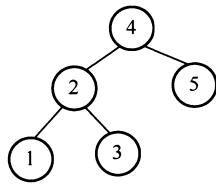
\includegraphics[width=0.3\textwidth]{images/44ce064387ffce4d8448abe51cc4936728a68a41ed0b614753e48d2dab29c57c.jpg}
\end{figure}

\choices{4,5,2,1,3}{4,5,1,2,3}{$4,2,5,3,1$}{4,2,1,3,5}

\begin{answersection}
B. 4,5,1,2,3
\end{answersection}

\begin{analysissection}
按照二叉排序树的插入规则，逐个插入序列中的元素。对于序列B：4,5,1,2,3，插入顺序为：4→5(右子树)→1(左子树)→2(1的右子树)→3(2的右子树)，这与图示的结构不符。
\end{analysissection}
\end{choicequestion}

\begin{choicequestion}[单选题]
\question{修改递归方式实现的图的深度优先搜索（DFS）算法，将输出（访问）顶点信息的语句移到退出递归前（即执行输出语句后立刻退出递归）。采用修改后的算法遍历有向无环图 $G$ ，若输出结果中包含 $G$ 中的全部顶点，则输出的顶点序列是 $G$ 的（）。}{B}
\choices{拓扑有序序列}{逆拓扑有序序列}{广度优先搜索序列}{深度优先搜索序列}

\begin{answersection}
B. 逆拓扑有序序列
\end{answersection}

\begin{analysissection}
修改后的算法在递归返回前输出顶点，这相当于在处理完一个顶点的所有后继节点后才输出该顶点。在DAG中，这意味着只有当一个顶点的所有可达顶点都被输出后，该顶点才被输出，这构成了逆拓扑序列。
\end{analysissection}
\end{choicequestion}

\begin{choicequestion}[单选题]
\question{已知无向图 $G$ 如下所示，使用克鲁斯卡尔（Kruskal）算法求图 $G$ 的最小生成树，加到最小生成树中的边依次是（ ）。}{A}

\begin{figure}[H]
\centering
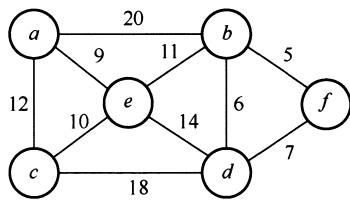
\includegraphics[width=0.3\textwidth]{images/769c67aa652b395b9bd0af93405b29f1cd180355b2882f0fbbdefe55bba5277d.jpg}
\end{figure}

\choices{$(b,f),(b,d),(a,e),(c,e),(b,e)$}{$(b,f),(b,d),(b,e),(a,e),(b,f)$}{$(a,e),(b,e),(c,e),(b,d),(b,f)$}{$(a,e),(c,e),(b,e),(b,f),(b,d)$}

\begin{answersection}
A. $(b,f),(b,d),(a,e),(c,e),(b,e)$
\end{answersection}

\begin{analysissection}
Kruskal算法按边权重从小到大排序，依次选择不形成环的边。根据图中边的权重，按此顺序选择边可以构建最小生成树。
\end{analysissection}
\end{choicequestion}

\begin{choicequestion}[单选题]
\question{若使用 AOE 网估算工程进度，则下列叙述中正确的是（）。}{B}
\choices{关键路径是从原点到汇点边数最多的一条路径}{关键路径是从原点到汇点路径长度最长的路径}{增加任一关键活动的时间不会延长工程的工期}{缩短任一关键活动的时间将会缩短工程的工期}

\begin{answersection}
B. 关键路径是从原点到汇点路径长度最长的路径
\end{answersection}

\begin{analysissection}
在AOE网中，关键路径是路径长度最长的路径，决定了整个工程的最短完成时间。关键活动的延迟会影响工期，但缩短非关键活动不能缩短工期。
\end{analysissection}
\end{choicequestion}

\begin{choicequestion}[单选题]
\question{下列关于大根堆（至少含 2 个元素）的叙述中，正确的是（）。\newline
I. 可以将堆视为一棵完全二叉树\newline
II. 可以采用顺序存储方式保存堆\newline
III. 可以将堆视为一棵二叉排序树\newline
IV. 堆中的次大值一定在根的下一层}{C}
\choices{仅 I、II}{仅 II、III}{仅 I、II 和 IV}{I、III 和 IV}

\begin{answersection}
C. 仅 I、II 和 IV
\end{answersection}

\begin{analysissection}
I. 正确，堆是完全二叉树。
II. 正确，堆常用数组存储。
III. 错误，堆不是二叉排序树。
IV. 正确，大根堆的次大值在根的左右子节点中。
\end{analysissection}
\end{choicequestion}

\begin{choicequestion}[单选题]
\question{依次将关键字 5, 6, 9, 13, 8, 2, 12, 15 插入初始为空的 4 阶 B 树后，根结点中包含的关键字是（）。}{A}
\choices{8}{6,9}{8, 13}{9, 12}

\begin{answersection}
A. 8
\end{answersection}

\begin{analysissection}
4阶B树的节点最多包含3个关键字，最少包含1个关键字（根节点）或⌈m/2⌉-1=1个关键字（非根节点）。
依次插入5,6,9,13,8,2,12,15，通过逐步构建过程可以确定最终根节点的关键字。
\end{analysissection}
\end{choicequestion}

\begin{choicequestion}[单选题]
\question{对大部分元素已有序的数组进行排序时，直接插入排序比简单选择排序效率更高，其原因是（）。\newline
I. 直接插入排序过程中元素之间的比较次数更少\newline
II. 直接插入排序过程中所需要的辅助空间更少\newline
III. 直接插入排序过程中元素的移动次数更少}{A}
\choices{仅 I}{仅 III}{仅 I、II}{I、II 和 III}

\begin{answersection}
A. 仅 I
\end{answersection}

\begin{analysissection}
对于已基本有序的数组，直接插入排序的比较次数会显著减少，因为内层循环会在较早的时候结束。但移动次数不一定更少，空间复杂度相同。
\end{analysissection}
\end{choicequestion}

\section{综合应用题}

\begin{choicequestion}[问答题]
\question{(13分)定义三元组 $(a,b,c)$ （其中 $a,b,c$ 均为正数）的距离 $D = |a - b| + |b - c| + |c - a|$ 。给定3个非空整数集合 $S_{1}$ 、 $S_{2}$ 和 $S_{3}$ ，按升序分别存储在3个数组中。设计一个尽可能高效的算法，计算并输出所有可能的三元组 $(a,b,c)$ （ $a\in S_1,b\in S_2,c\in S_3$ ）中的最小距离。例如 $S_{1} = \{-1,0,9\}$ ， $S_{2} = \{-25, - 10,10,11\}$ ， $S_{3} = \{2,9,17,30,41\}$ ，则最小距离为2，相应的三元组为(9,10,9)。要求：\newline
1）给出算法的基本设计思想。  \newline
2）根据设计思想，采用C或 $\mathrm{C + + }$ 语言描述算法，关键之处给出注释。  \newline
3）说明你所设计算法的时间复杂度和空间复杂度。}{}

\begin{answersection}
1）算法的基本设计思想：
使用三指针技术。由于三个数组已按升序排列，我们可以使用三个指针分别指向三个数组的当前位置。对于当前三元组，计算其距离。为了减小距离，我们应该移动最大值或最小值对应的指针（使其更靠近中间值）。重复此过程直到某个指针超出边界。

2）算法实现：
\end{answersection}

\begin{analysissection}
#include <stdio.h>
#include <stdlib.h>
#include <limits.h>
#include <math.h>

int minDistance(int* S1, int size1, int* S2, int size2, int* S3, int size3) {
    int i = 0, j = 0, k = 0;  // 三个指针
    int minDist = INT_MAX;
    
    while (i < size1 && j < size2 && k < size3) {
        int a = S1[i], b = S2[j], c = S3[k];
        int dist = abs(a - b) + abs(b - c) + abs(c - a);
        minDist = (dist < minDist) ? dist : minDist;
        
        // 移动最小值对应的指针
        if (a <= b && a <= c) {
            i++;
        } else if (b <= a && b <= c) {
            j++;
        } else {
            k++;
        }
    }
    
    return minDist;
}

3）时间复杂度：O(n1 + n2 + n3)，其中n1, n2, n3分别是三个数组的长度。空间复杂度：O(1)，只使用了常数个额外变量。
\end{analysissection}
\end{choicequestion}

\begin{choicequestion}[问答题]
\question{(10分)若任一个字符的编码都不是其他字符编码的前缀，则称这种编码具有前缀特性。现有某字符集（字符个数 $\geq 2$ ）的不等长编码，每个字符的编码均为二进制的0、1序列，最长为 $L$ 位，且具有前缀特性。请回答下列问题：\newline
1）哪种数据结构适宜保存上述具有前缀特性的不等长编码？  \newline
2）基于你所设计的数据结构，简述从0/1串到字符串的译码过程。  \newline
3）简述判定某字符集的不等长编码是否具有前缀特性的过程。}{}

\begin{answersection}
1）适宜使用Trie树（前缀树）保存具有前缀特性的编码。

2）译码过程：从Trie树的根节点开始，按位扫描0/1串，遇到0则走向左子树，遇到1则走向右子树，直到到达叶子节点，输出该叶子节点对应的字符，然后回到根节点继续处理后续的0/1串。

3）判定过程：对于所有编码，检查是否有一个编码是另一个编码的前缀。可以通过构建Trie树来判断，如果某个非叶子节点存储了字符，则说明存在前缀关系，不具有前缀特性。
\end{answersection}

\begin{analysissection}
1）Trie树（字典树）是保存前缀码的理想数据结构，它能够有效地表示具有前缀特性的编码集。

2）译码过程：
- 从Trie树根节点开始
- 依次读取二进制串的每一位
- 如果是'0'，向左子节点移动；如果是'1'，向右子节点移动
- 当到达标记为字符结束的节点时，输出对应字符
- 回到根节点，继续处理后续的二进制位

3）判定前缀特性的过程：
- 方法一：对每一对编码，检查其中一个是否是另一个的前缀
- 方法二：构建Trie树，如果某个路径上的非叶子节点（非末端节点）包含字符标识，则说明不具有前缀特性
- 方法三：按编码长度排序后，只需检查较短编码是否为较长编码的前缀
\end{analysissection}
\end{choicequestion}

\end{document}